\documentclass{"../res/univ-projet"}
\usepackage[latin1]{inputenc}
\usepackage[T1]{fontenc}
\usepackage[francais]{babel}

\title{Sp�cification Technique des Besoins}
\author{\bsc{Michotte} Maxime}
\projet{M1SSI}
\projdesc{Projet de g�n�ration d'OTP}
\filiere{M1SSI}
\version{1.0}
\relecteur{\bsc{Zigh} Benjamin}
\signataire{\bsc{Bardet} Magali}
\date{Novembre 2013}

\histentry{1.0}{15/11/2013}{test}

\begin{document}
\maketitle
%-------------------------------------------------------------------------------
\section*{Objet}
Etude et impl�mentations des syst�mes d'authentification utilisant des mots de passe jetables :
\begin{itemize}
    \item Besoin op�rationnel
        \begin{itemize}
            \item Garantir une authentification forte
            \item Etat de l'art sur les syst�mes existants
            \item Objectif : mise en production
        \end{itemize}
    \item Objectifs techniques
	    \begin{itemize}	
            \item Impl�mentation des solutions retenues sur un ou plusieurs supports
	    \end{itemize}
    \item Contraintes et recommmandations
        \begin{itemize}
            \item Respecter les sp�cifications de base et norme RFC
            \item Montrer que le syst�me produit est s�r
            \item Choisir une impl�mentation adapt�e en fonction des besoins et de l'�tat de l'art �tablie
        \end{itemize}
    \item R�sultats attendus
        \begin{itemize}
            \item Syst�me s�r et fonctionnel
            \item Etat de l'art le plus exhaustif possible
            \item Impl�mentation sur Carte � puces et/ou Android
        \end{itemize}
\end{itemize}
%-------------------------------------------------------------------------------
\section*{Documents applicables et de r�f�rence}
\begin{itemize}
    \item \href{http://tools.ietf.org/html/rfc2289}{RFC 2289}, \href{http://www.ietf.org/rfc/rfc4226.txt}{RFC 4226}, \href{http://www.ietf.org/rfc/rfc4256.txt}{RFC 4256}, \href{http://tools.ietf.org/html/rfc4793}{RFC 4793}, \href{http://tools.ietf.org/html/rfc6238}{RFC 6238}
	\item \href{http://code.google.com/p/google-authenticator/}{Google Authenticator}
\end{itemize}
%-------------------------------------------------------------------------------
\section*{Terminologie et sigles utilis�s}
	- 
%-------------------------------------------------------------------------------
\section*{Exigence fonctionnelles}
\begin{figure}
\hfill
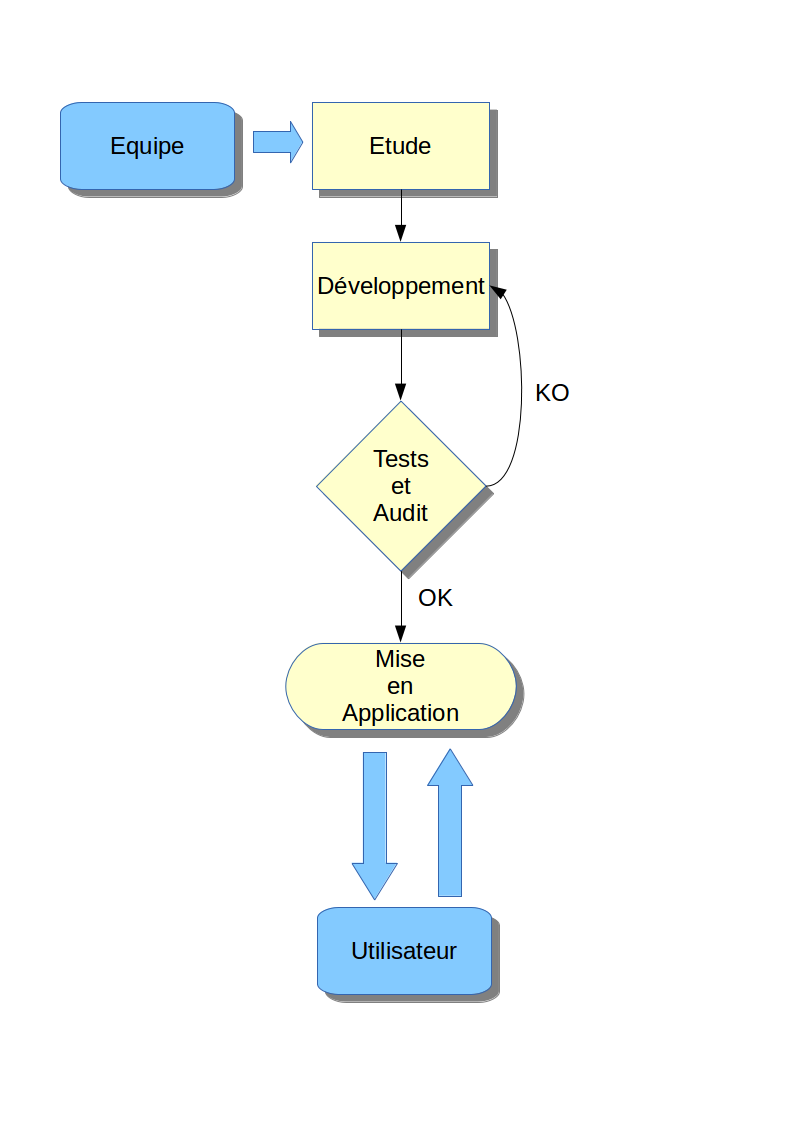
\includegraphics[scale=0.5]{diagramme1.png}
\hfill
\caption{Sch�ma}
\end{figure}
\begin{tabular}{|c|l|l|c|}
    \hline
    \rowcolor{gray}
    \textcolor{white}{Id} & \textcolor{white}{Intitul�} & \textcolor{white}{Acteur(s)} & \textcolor{white}{Priorit�}\\
    \hline
    1 & Etat de l'art & Equipe & Indispensable\\
    \hline
    2 & Association & Client & Indispensable\\
    \hline
    3 & G�n�ration & Client & Indispensable\\
    \hline
    4 & Authentification & Client & Indispensable\\
    \hline
    5 & Re-synchronisation & Equipe & Indispensable\\
    \hline
\end{tabular}
	
%-------------------------------------------------------------------------------
\section*{Exigences op�rationnelles}
\begin{tabular}{|c|l|c|}
    \hline
    \rowcolor{gray}
    \textcolor{white}{Id} & \textcolor{white}{Intitul�} & \textcolor{white}{Priorit�}\\
    \hline
    EF\_01 & G�n�ration d'un OTP en moins d'une secondes & Indispensable\\
    \hline
    EF\_02 & OTP non pr�visible & Indispensable\\
    \hline
    EF\_03 & R�sistant � une attaque exhaustive & Indispensable\\
    \hline
    EF\_04 & Respect des RFC & Indispensable\\
    \hline
\end{tabular}

%-------------------------------------------------------------------------------
\section*{Exigences d'interface}
\begin{tabular}{|c|l|c|}
    \hline
    \rowcolor{gray}
    \textcolor{white}{Id} & \textcolor{white}{Intitul�} & \textcolor{white}{Priorit�}\\
    \hline
    E\_INT01 & UNIX(Client/Serveur/Token) & Indispensable\\
    \hline
    E\_INT02 & Android(Token) & Important\\
    \hline
    E\_INT03 & Java Card & Secondaire\\
    \hline
\end{tabular}

%-------------------------------------------------------------------------------
\section*{Exigences de qualit�}

%-------------------------------------------------------------------------------
\section*{Exigences de r�alisation}

%-------------------------------------------------------------------------------
\end{document}
